% Please make sure you insert your
% data according to the instructions in PoSauthmanual.pdf
\documentclass{PoS}

\title{Diffractive PDF determination from HERA inclusive and jet data at NNLO QCD}

\ShortTitle{Diffractive PDF determination from HERA inclusive and jet data at NNLO QCD}

\author{\speaker{Radek \v{Z}leb\v{c}\'{i}k}\\ on behalf of the \textup{\textbf{H1 Collaboration}} \\
        DESY\\
        E-mail: \email{radek.zlebcik@desy.de}}

%\author{Another Author\\
%        Affiliation\\
%        E-mail: \email{...}}


%\usepackage[utf8]{inputenc}
\usepackage{xspace}
\usepackage{amsmath}
\usepackage{amssymb}



\newcommand{\IP}{I\!\!P}
\newcommand{\IR}{I\!\!R}
\newcommand{\xpom}{x_{\IP}}

\newcommand{\GeV}{\ensuremath{\mathrm{GeV}}\xspace}
\newcommand{\GeVsq}{\ensuremath{\mathrm{GeV}^2}\xspace}

%\newcommand{\includegraphicss} 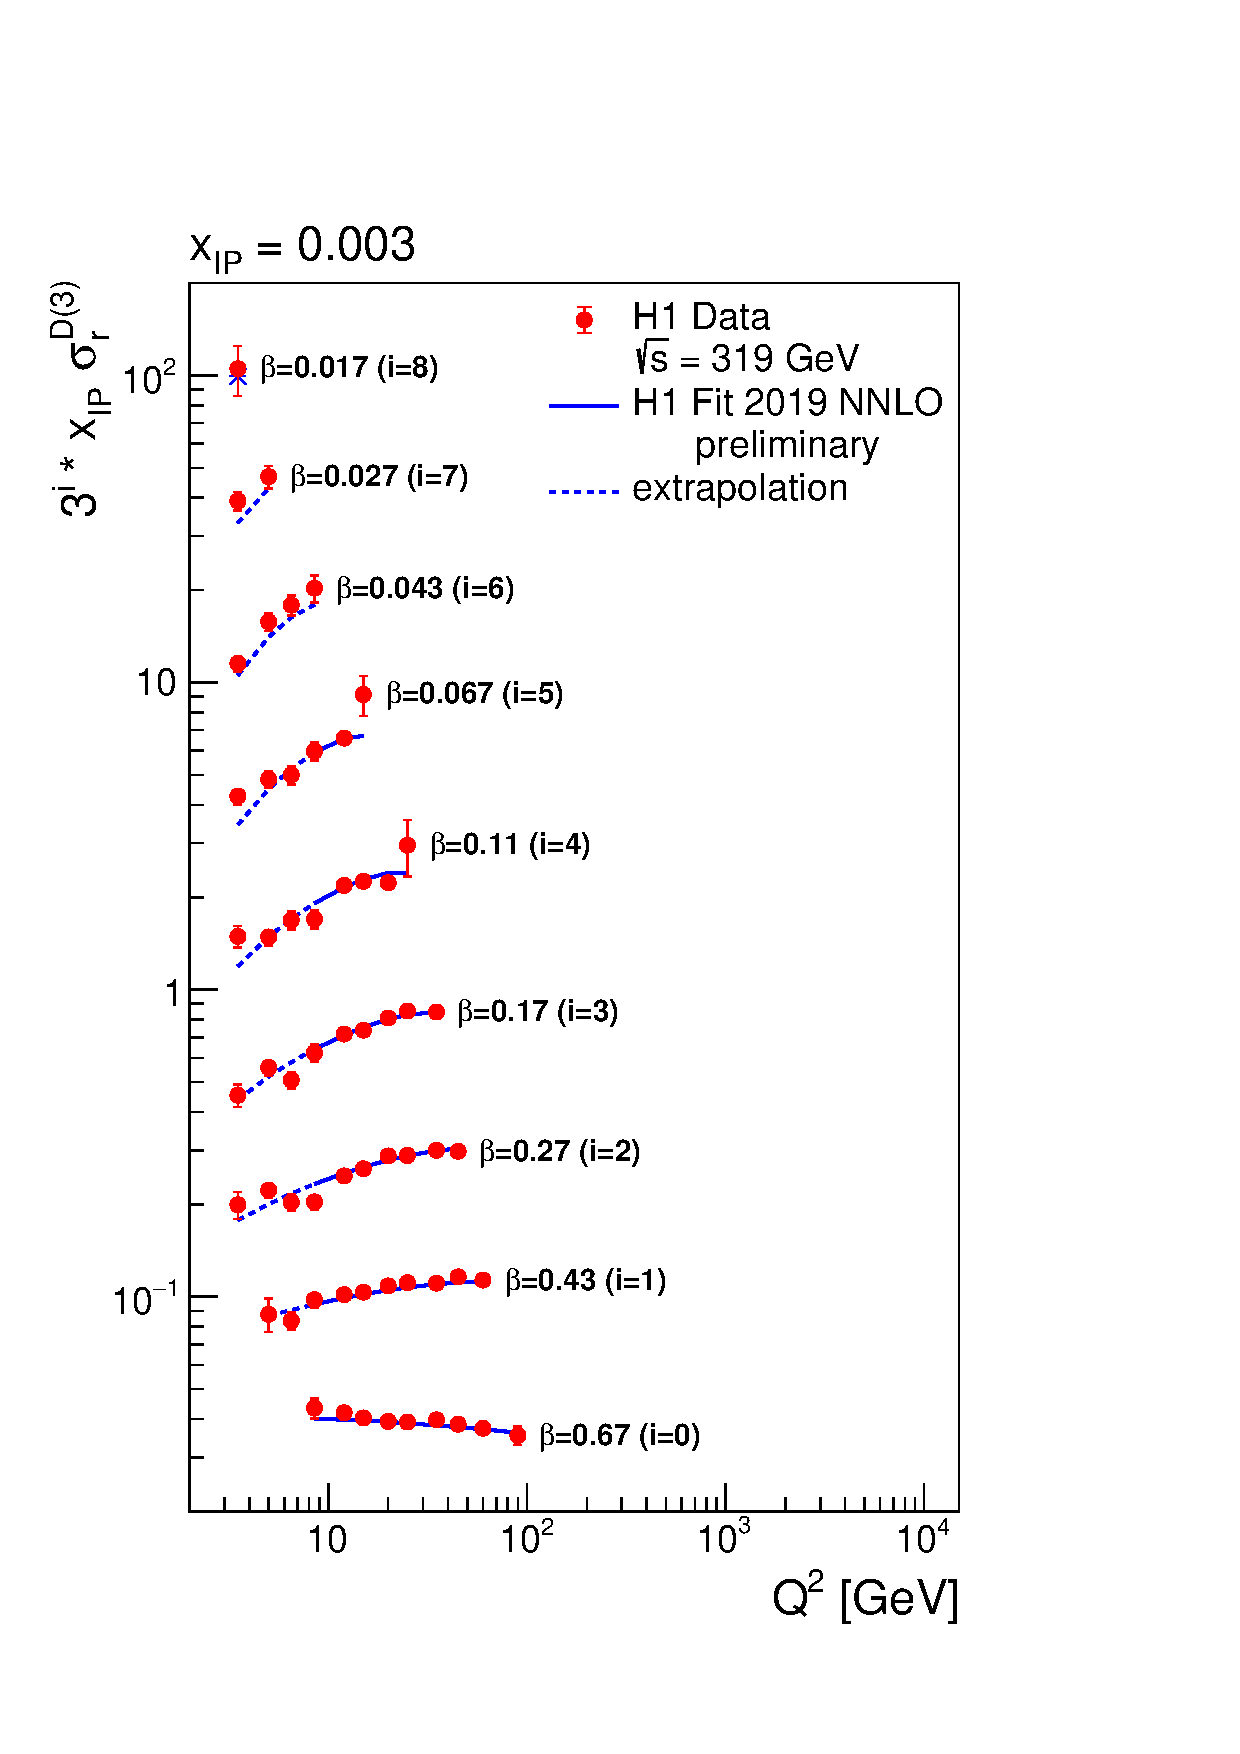
\includegraphics[width=.9\textwidth]{{{plots/H1prelim-19-013.fig10}}}

\newcommand{\includegraphicss}[2][]{\fbox{\includegraphics[#1]{#2}}}
%            Mandatory arg: #2; Optional arg: #1.}


\abstract{A new fit of diffractive parton distribution functions (DPDFs) to the HERA inclusive and jet data in diffractive deep-inelastic scattering (DDIS) at next-to-next-to-leading order accuracy (NNLO) is presented. The inclusion of the most comprehensive dijet cross section data, together with their NNLO predictions, provide enhanced constraint to the gluon component of the DPDF, which is of particular importance for diffractive PDFs. Compared to previous HERA fits, the presented fit includes the high-precision HERA~II data of the H1 collaboration, which corresponds to a 40-fold increase in luminosity for inclusive data (six-fold increase for jet data). In addition to the inclusive sample at nominal centre-of-mass energy $\sqrt{s} = 319\,\GeV$, inclusive H1 data at $252$~GeV and $225$~GeV are included. The extracted DPDFs are compared to previous DPDF fits, and are used to predict cross sections for a large number of available measurements and differential observables.}

\FullConference{XXVII International Workshop on Deep-Inelastic Scattering and Related Subjects - DIS2019\\
		8-12 April, 2019\\
		Torino, Italy}


\begin{document}

\section{Introduction}

Diffractive processes, $ep \to  eXY$, where the systems $X$ and $Y$ are separated in rapidity, have been studied extensively at the electron-proton collider HERA.
The forward system $Y$ usually consists of the leading proton but can also contain its low mass dissociation.
Between the systems $X$ and $Y$ is a depleted region without any hadronic activity (large rapidity gap) which is a consequence of the vacuum quantum numbers of the diffractive exchange, often referred to as a pomeron ($\IP$).
Experimentally, diffractive events can be selected either by requiring a rapidity region without any hadronic activity, large rapidity gap (LRG) method , or by direct detection of the leading proton.
In the second case, the system $Y$ is free of any diffractive dissociation.

In analogy to the non-diffractive case, also in diffraction parton distribution functions can be defined.
According to the factorisation theorem \cite{Collins:1997sr} the diffractive cross section is then expressed as a convolution of these diffractive densities (DPDFs) and partonic cross sections of the hard subprocess which are calculable within perturbative QCD.
The DPDFs have properties similar to the classical PDFs, especially they obey the DGLAP evolution equation, but have an additional constraint on the presence of the leading proton in the final state.
Within the diffractive factorisation frame the DPDFs are extracted from the reduced cross sections of inclusive diffractive DIS \cite{Aktas:2006hy} which is the process with the highest statistics.
Consequently these DPDFs are used to predict cross sections of other, more exclusive, processes in DIS.
At HERA, due to relatively small masses of system $X$, only the dijet cross sections and $D^{*}$ cross sections were measured.
As the gluonic component of DPDFs is weakly constrained from the inclusive measurement both H1 and ZEUS collaborations performed also a combined fit of inclusive and dijet data \cite{Aktas:2007bv,Chekanov:2009aa} where the dijet cross section allows for a better constraint of the gluon DPDF component.
So far all these DPDF extractions were performed at the NLO order of the pQCD and they suffered from large QCD scale uncertainties of the predictions for dijet cross section.

In the \cite{Britzger:2018zvv} the NNLO predictions for the dijet production in DDIS were presented.
It was observed that NNLO predictions lead to about twice smaller theoretical uncertainties compared to NLO, however, the NNLO predictions in general overshoot the measured cross section.
Since only NLO DPDFs were available at that time, we believed that the difference can be explained by inconsistency between pQCD order in the PDFs and in the matrix elements.


We present a combined QCD fit at NNLO of inclusive and dijet data.
This new fit benefits from both, from more precise theory as well as from HERA II data sets, which were not available when previous H1 fits originated.
To test the factorization theorem, extracted DPDFs are then used to predict the dijet cross sections for several analyses not included in the fit. 
In this way all the calculations are done consistently at NNLO.


\section{Variable definition}
The standard DIS observables are the photon virtuality $Q^2 = −q^2$ ($q = k - k'$), the inelasticity $y$ defined as $y = \frac{pq}{pk}$ and $x$-Bjorken, $x_\mathrm{bj}$ ($x_\mathrm{bj}=\frac{Q^2}{sy}$), where the incoming proton four-momentum is labeled as $p$ and $k$ ($k'$) denotes the incoming (scattered) electron four-momentum. 
For diffractive processes additional kinematic variables $x_{\IP}$ and  $t$ describing the scattered proton are introduced.
The variable $x_{\IP}$ is a relative energy loss of the beam proton caused by the diffractive scattering and $t$ approximately equals to  $-p_T^2$, where $p_T$ is the transverse momentum of the scattered proton.

The cross sections are studied differentially in several kinematic variables which are also used to constrain the phase space of the measurement.
The jets in case of dijet analyses were identified using the $k_T$-algorithm in the $\gamma^{∗}p$ frame with the distance parameter $R = 1$ and their transverse momentum or pseudo-rapidity were measured either in $\gamma^{*}p$ or in the laboratory frame.

Notice, that at LO for inclusive (dijet) production the variable $\beta = \frac{x_\mathrm{bj}}{x_{\IP}}$ ($z^\mathrm{obs}_{\IP} = \frac{M_{12}^2 + Q^2}{M_X^2 + Q^2}$) can be interpreted as a momentum fraction of parton entering hard sub-process w.r.t. the diffractive exchange momentum.



\section{Fitting procedure}

We fit the data from combined HERA~I and HERA~II measurement of the inclusive reduced diffractive cross section $\sigma_r^{D(3)}(\xpom, Q^2, \beta)$  at the nominal HERA centre-of-mass energy $\sqrt{s} = 319\,\GeV$ and luminosity up to $\sim\!\! 340\,\text{pb}^{-1}$  \cite{Aaron:2012ad}.
Also the inclusive data from low-energy HERA~II runs at $\sqrt{s} = 225\,\GeV$ ($8.5\,\text{pb}^{-1}$) and $\sqrt{s} = 252\,\GeV$ ($5.2\,\text{pb}^{-1}$) are included \cite{Aaron:2012zz}.
In addition the DPDF fit is constrained by the DDIS dijet data, where the 2D ($p_T^{\mathrm{jet}1}$, $Q^2$) spectrum is included in the combined fit \cite{Andreev:2014yra}.
Only the inclusive diffractive data satisfying $Q^2 > 8.5 \GeVsq$ and $\beta < 0.8$ and $M_X = \sqrt{Q^2(1/\beta - 1)} > 2\,\GeV$ are fitted to avoid problematic region of the phase space where pQCD predictions are not reliable, similarly as in \cite{Aktas:2006hy}.
All these data sets are based on the Large Rapidity Gap method selecting the diffractive events with $|t| < 1\,\GeVsq$ and $M_Y < 1.6\,\GeVsq$.


The input DPDF parametrization at the starting scale has the following form (Regge factorization ansatz):
\begin{equation}
f_i (z, \mu^2, \xpom, t) = f_{i/\IP} (z, \mu^2) f_{\IP/p} (\xpom, t) + n_{\IR} f_{i/\IR} (z, \mu^2) f_{\IR/p} (\xpom, t),
\end{equation}
where the "Pomeron PDF" at the starting scale  $f_{i/\IP}(z, \mu_0^2)$ is supposed to be equal for all light flavours $i=u=d=s = \bar{u} = \bar{d} = \bar{s}$, whereas the heavy flavours are produced through the DGLAP evolution.
The parametrization form for both light quarks and gluon of the Pomeron PDF has equal form $A z^B (1-z)^C$.
The second term corresponding to so called "Reggon PDF" is only important at higher $\xpom$ and is fixed to be equal to the pion PDF \cite{Owens:1984zj}.

The parameters  $\alpha_{\IR}(0)$,  $\alpha'_{\IR}$, $B_{\IR}$   of the Reggeon flux are kept the same as in the previous H1 fits \cite{Aktas:2006hy,Aktas:2007bv}, whereas the Pomeron flux parameters $\alpha'_{\IP}$, $B_{\IP}$ are updated to their latest values extracted from FPS HERA~II data \cite{Aaron:2010aa}, i.e. $\alpha'_{\IP} = 0.04^{+0.08}_{-0.06}$ and\footnote{The uncertainties of the quoted parameters are propagated into uncertainties of the DPDFs.} $B_{\IP} = 5.74^{+0.84}_{-0.93}$.
The Pomeron intercept $\alpha_{\IP}(0)$ and the overall normalization of the Reggeon term $n_{\IR}$ are considered as a free parameters and are extracted from the presented fit.
In total there are 8 parameters to be fitted, $A_q$, $B_q$, $C_q$, $A_g$, $B_g$, $C_g$, $\alpha_{\IP}(0)$ and $n_{\IR}$.


From the starting scale $\mu_0 = 1.15\,\GeV$ the DPDFs were evolved to the higher values using DGLAP evolution equations with GM-VFNS at NNLO as implemented in \cite{Botje:2010ay,Bertone:2013vaa}.
The value of the strong coupling is set to be $\alpha_S^{N_f = 5} (M_Z) = 0.118\pm 0.002$ and the charm and bottom masses to $m_c = 1.4\pm 0.2$, $m_b = 4.5\pm 0.5$.
The inclusive reduced cross section $\sigma_r^D$ is evaluated in the FONLL-C flavour scheme \cite{Cacciari:1998it} as implemented in the APFEL package \cite{Bertone:2013vaa}.
The predictions for the dijet production in DDIS are based on NNLOJET program \cite{Currie:2016ytq} which employs an antenna subtraction method.
The renormalization and factorization scales are set to be identical and equal to $Q^2$ in case of inclusive DDIS and $Q^2 + \langle p_T\rangle^2$ for dijet production.
The scale uncertainty is estimated by varying renormalization and factorization scales simultaneously by a factor of 2.

We employ the fastNLO method \cite{Britzger:2012bs} which allows fast recalculation of the cross sections when the fitted or model parameters are varied.
The fit itself is performed using Alpos fitting framework \cite{yyy}.

\section{Results of the fit}

The examples of the fitted distributions (for $x_{\IP} = 0.001$ and $x_{\IP} = 0.003$) can be seen in Fig.~\ref{figDDISfit}.
% DDIS data fitted
\begin{figure}[h]
\centering
\begin{minipage}[t]{0.47\textwidth}
\includegraphicss[trim={0cm 0.0cm 0 0.0cm},clip,width=.9\textwidth]{{{plots/H1prelim-19-013.fig11}}}
\end{minipage}
\begin{minipage}[t]{0.47\textwidth}
\includegraphicss[trim={0cm 1.2cm 0 1.1cm},clip,width=.9\textwidth]{{{plots/H1prelim-19-013.fig10}}}
\end{minipage}
\caption{The reduced DDIS cross sections, $x_{\IP}\sigma_r^{D(3)}$, as measured by the H1 collaboration (red bullets with error bars denoting the overall experimental uncertainty). These data are fitted by NNLO pQCD predictions denoted by the blue line. The line is hashed for data points not included into the fit, where the prediction is only extrapolated.}
\label{figDDISfit}
\end{figure}
In general all fitted data sets are well described by the fitted theory, as can be seen from the obtained $\chi^2/n_\mathrm{pt}$ values, which are $192/191$ ($29/25$) for inclusive DDIS at nominal (reduced) beam energy and $12/15$ for the dijet production in DDIS.
In total $\chi^2/n_\mathrm{df} = 235/223$.

The obtained DPDFs are labeled as H1~Fit2019 NNLO and in Fig.~\ref{figDPDF} they are compared to the H1~Fit2006B NLO \cite{Aktas:2006hy}.
% DPDF plot
\begin{figure}[h]
\centering
\includegraphicss[trim={0cm 0.5cm 0 1.5cm},clip,width=.7\textwidth]{{{plots/H1prelim-19-013.fig1}}}
\caption{ Singlet (left, $\Sigma$) and gluon (right, $g$) distributions of the Pomeron in H1~Fit2019 NNLO (prel.) as a function of $z$ for three different values of $µ$ at a value of $x_{\IP} = 0.003$. The inner (dark) error band displays the experimental uncertainty, while the outer (bright) error band displays the full uncertainty, i.e. experimental, parameterisation, model and theoretical uncertainties added in quadrature. The H1~Fit2019~NNLO (prel.) is compared to H1~Fit2006B (dashed line), which was obtained in an NLO pQCD fit.}
\label{figDPDF}
\end{figure}
%
It can be seen that the singlet part is similar for both fits since the quark distribution is well constrained by the inclusive data, whereas the gluon contribution which is more sensitive to the higher-order effects is about 30\% smaller for the new fit.


\section{Predictions based on new NNLO DPDF}

We calculated the theoretical cross sections for several measurements of the dijet production made by H1 and ZEUS collaborations.
For a comparison, the new H1~Fit2019 NNLO as well as older H1~Fit2006B NLO DPDFs \cite{Aktas:2006hy} were used for the predictions.

In the Fig.~\ref{figTotalXsecs} we observe that the new fit describes the overall data normalization better than the H1~Fit2006B, where NLO DPDF is convoluted with NNLO partonic cross sections.
%
\begin{figure}[h]
\centering
\includegraphicss[trim={0cm 1.7cm 0 0.7cm},clip,width=.6\textwidth]{{{plots/H1prelim-19-013.fig3}}}
\caption{ NNLO pQCD predictions (full blue line) using H1 Fit2019 NNLO (prel.) in comparison to the total dijet cross section measured in six different analysis by the H1 or ZEUS collaborations (full circles). The upper panel displays the total cross section, and the lower panel the ratio of the predictions to data. The inner error band (dark blue) displays the DPDF uncertainty of the H1 Fit2019 NNLO (prel.) fit, and the outer error band (light blue) displays the DPDF uncertainty and scale uncertainty added in quadrature. The hatched band displays the DPDF uncertainty and NLO scale uncertainty of the NLO predictions. The inner error of the data displays the statistical uncertainty, and the full error bars displays the total experimental uncertainty. For comparison, NNLO pQCD predictions using the H1~Fit2006B NLO PDF are also shown.}
\label{figTotalXsecs}
\end{figure}
%
The description of the individual measurements and the references to corresponding publications can be found in \cite{Britzger:2018zvv}.
Only the normalization of the H1 HERA~I analyses is a bit overshot.
To be noted, the "H1 LRG (HERA~II)" data differential in $p_T^{\mathrm{jet}1}$ and $Q^2$ were included into the QCD fit described in the previous session.

In addition to the total cross section, several differential distributions were also studied.
As an example, in Fig.~\ref{figZEUSdiff} the differential distributions as measured by the ZEUS collaboration, i.e. "ZEUS LRG (HERA~I)", are compared to the predictions.
\begin{figure}[h]
\centering
\includegraphicss[trim={0cm 0.3cm 0 0.3cm},clip,width=.8\textwidth]{{{plots/H1prelim-19-013.fig7}}}
\caption{ NNLO pQCD predictions (full blue line) using H1 Fit2019 NNLO (prel.) for the dijet production in DDIS compared to the experimental data from ZEUS collaboration (full circles). The upper panels display the differential distributions as a function of $z_{\IP}^\mathrm{obs}$, $Q^2$, $p_T^\mathrm{jets}$ and $\eta^{*\mathrm{jets}}$, and the lower panel the ratio of the predictions to data. The inner error band (dark blue) displays the DPDF uncertainty of the H1 Fit2019 NNLO (prel.) fit, and the outer error band (light blue) displays the DPDF uncertainty and scale uncertainty added in quadrature. The hatched band displays the DPDF uncertainty and NLO scale uncertainty of the NLO predictions. The inner error of the data displays the statistical uncertainty, and the full error bars displays the total experimental uncertainty. For comparison, NNLO pQCD predictions using the H1~Fit2006B NLO DPDF are also shown.}
\label{figZEUSdiff}
\end{figure}
As already seen in the plot with total cross sections the newer NNLO fit describes the overall normalization better, the quality of the shape description is comparable for both DPDFs.

\section{Conclusion}
The present the fist QCD analysis of the DDIS data at NNLO of the perturbative theory.
The NNLO DPDFs were extracted from the combined fit of inclusive and dijet DDIS data.
To test the factorization the extracted DPDF was used to predict cross sections for other dijet measurement.
We observed good description of the data points by NNLO predictions based on NNLO DPDFs, compared to predictions based on previous H1 DPDF fits, which overshoot the data.


\bibliographystyle{JHEP}
\bibliography{refs}


\end{document}



